% !TEX root = ./proj_report.tex
\graphicspath{{mehul_pics/}}% Set graphics path location
\subsection{Filter Mathematical Theory} %\label{sec:appendix}
% !TEX root = ./proj_report.tex
This section presents the mathematical formulation of the chosen filters. Filter kernels are defined by $G(\omega_1,\omega_2)$ which is the discrete Fourier transform (DFT) of $g(m,n)$. Recollect that restored image in the Fourier domain can be mathematically represented as,
\begin{equation}
v(m,n)= h(m,n) \star u(m,n) + \eta(m,n)
\end{equation}
\begin{equation}
DFT(h(m,n)) = H(\omega_1,\omega_2)
\end{equation}
\begin{equation}
\hat{U}(\omega_1,\omega_2)= G(\omega_1,\omega_2)V(\omega_1,\omega_2)
\end{equation}

\begin{enumerate}
\item {\bf Inverse Filter}\\
Most intuitive and easiest to implement filters. Unfortunately, these don't work so well when the image has noise.
\begin{equation}
G(\omega_1,\omega_2) = 1/H(\omega_1,\omega_2)
\end{equation}

\item {\bf Wiener Filter}\\
Very good with noisy images. Finite impulse response avoids working with large DFTs. Needs an estimate of the signal to noise ratio.
\begin{equation}
G(\omega_1,\omega_2) = \frac{H^*(\omega_1,\omega_2)}{|H(\omega_1,\omega_2)|^2 + \frac{S_{vv}}{S_{\eta\eta}}}
\end{equation}

\item {\bf Geometric mean Filter}\\
Another Fourier domain filter. Has the flexibility of choosing parameter {\sl s}. {\sl s} $\in$ [0,1]
\begin{equation}
G(\omega_1,\omega_2) = (H^-)^s\Bigl[\frac{H^*(\omega_1,\omega_2)}{|H(\omega_1,\omega_2)|^2 + \frac{S_{vv}}{S_{\eta\eta}}}\Bigr]^{1-s}
\end{equation}

\item {\bf Constrained Least Squares Filter}\\
Used MatLab's inbuilt function for this filter. Q is DFT of a predefined matrix and $\gamma$ is obtained through a solution of linear equations.
\begin{equation}
G_{ls}(\omega_1,\omega_2) = \frac{H^*(\omega_1,\omega_2)}{|H(\omega_1,\omega_2)|^2 + \gamma|Q(\omega_1,\omega_2)|^2}
\end{equation}

\item {\bf Filter + edge detection}\\
This is not really a filtering technique. We tried using one of the regular filters mentioned above and combine it with edge detection method to see if the combined image does better in sharpness metric. It wasn't successful in the first attempt and we didn't pursue it further. 
\begin{figure}[H]
\centering
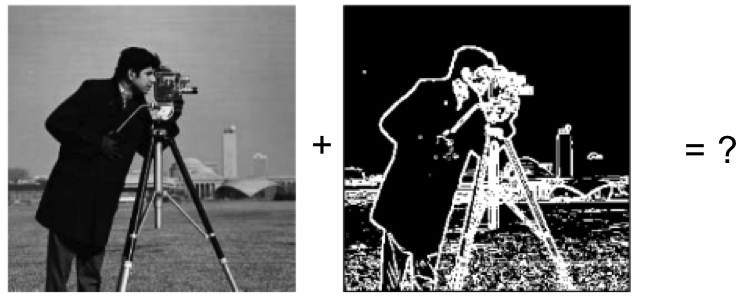
\includegraphics[scale=1]{ED}
\caption{Filter sharpened image + Edge detection == better sharp image ?}
\end{figure}

\end{enumerate}
\newpage